%
% The first command in your LaTeX source must be the \documentclass command.
\documentclass[sigconf]{acmart}

%
% defining the \BibTeX command - from Oren Patashnik's original BibTeX documentation.
\def\BibTeX{{\rm B\kern-.05em{\sc i\kern-.025em b}\kern-.08emT\kern-.1667em\lower.7ex\hbox{E}\kern-.125emX}}
    
% Rights management information. 
% This information is sent to you when you complete the rights form.
% These commands have SAMPLE values in them; it is your responsibility as an author to replace
% the commands and values with those provided to you when you complete the rights form.
%
% These commands are for a PROCEEDINGS abstract or paper.

\copyrightyear{2019}
\acmYear{2019}
\setcopyright{acmlicensed}
\acmConference[CS 184 Sp19]{CS 184 Sp19: Final Project}{April 30, 2019}{Berkeley, CA}
\acmBooktitle{CS 184 Sp19: Final Project, April 30, 2019, Berkeley, CA}
\acmDOI{}

%
% These commands are for a JOURNAL article.
%\setcopyright{acmcopyright}
%\acmJournal{TOG}
%\acmYear{2018}\acmVolume{37}\acmNumber{4}\acmArticle{111}\acmMonth{8}

%\acmDOI{10.1145/1122445.1122456}

%
% Submission ID. 
% Use this when submitting an article to a sponsored event. You'll receive a unique submission ID from the organizers
% of the event, and this ID should be used as the parameter to this command.
%\acmSubmissionID{123-A56-BU3}

%
% The majority of ACM publications use numbered citations and references. If you are preparing content for an event
% sponsored by ACM SIGGRAPH, you must use the "author year" style of citations and references. Uncommenting
% the next command will enable that style.
%\citestyle{acmauthoryear}

%
% end of the preamble, start of the body of the document source.
\begin{document}

%
% The "title" command has an optional parameter, allowing the author to define a "short title" to be used in page headers.
% The "title" command has an optional parameter, allowing the author to define a "short title" to be used in page headers.
\title{Diffuse Relativistic Black Hole in the Cornell Box}

%
% The "author" command and its associated commands are used to define the authors and their affiliations.
% Of note is the shared affiliation of the first two authors, and the "authornote" and "authornotemark" commands
% used to denote shared contribution to the research.
\author{Andrew Aikawa}

\author{Yuan Zhou}

\author{Weylan Wang}

% The abstract is a short summary of the work to be presented in the article.
\begin{abstract}
We report a ray tracing algorithm in which we can quantitatively generate realistic images in a scene with a black hole.  The problem of illustrating what a black hole would look like has been explored previously in works such as the movie Interstellar\cite{james_tunzelmann_franklin_thorne_2015}. However, almost all of these assume purely emissive light sources and very distant light sources that would be represented as environment maps.  In this paper, we present a ray tracer for a scene with a Schwarzchild black hole in diffuse lighting conditions.
\end{abstract}


%
% Keywords. The author(s) should pick words that accurately describe the work being
% presented. Separate the keywords with commas.
\keywords{ray tracing, black holes, general relativity}

%
% A "teaser" image appears between the author and affiliation information and the body 
% of the document, and typically spans the page. 
\begin{teaserfigure}
  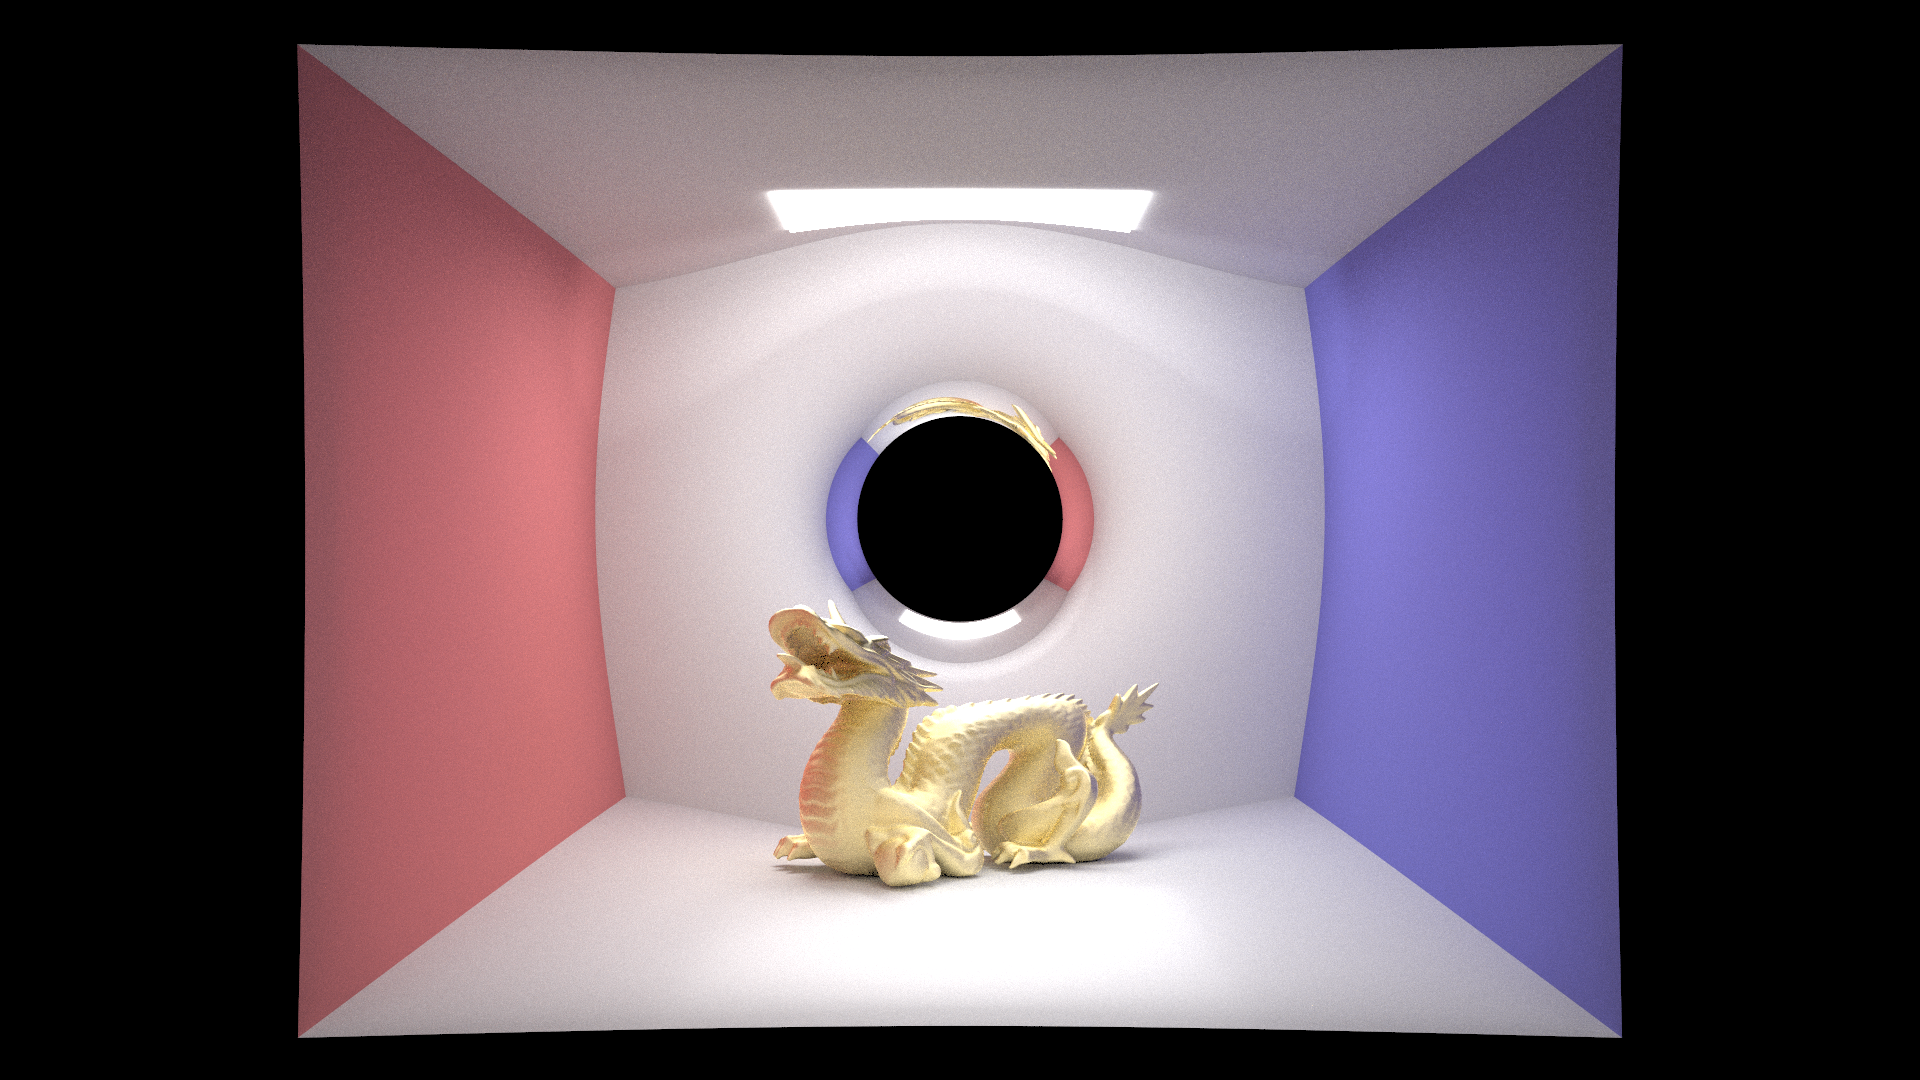
\includegraphics[width=\textwidth]{dragon.png}
  \caption{Gold Dragon in Cornell Box Containing a Black Hole}
  \Description{Gold Dragon in Cornell Box Containing a Black Hole}
  \label{fig:teaser}
\end{teaserfigure}

%
% This command processes the author and affiliation and title information and builds
% the first part of the formatted document.
\maketitle

\section{Ray Tracing in General Relativity}

Einstein's field equations predict changes in the spacetime curvature in the vicinity of a black hole. The metric tensor, $g_{\mu\nu}$, the solution to the field equations, determines the metric, how 'distance' is measured in spacetime. The path taken by a ray of light is determined by Fermat's principle, dictating that the ray will take whatever path takes the ray from point A to point B with the least action, a quantity describing how much metric distance the ray has traveled. In a typical Euclidean metric space, where the metric is uniform over all space and in a medium with a uniform index of refraction, rays will trace lines, a central assumption in traditional ray tracing algorithms. However, in the presence of a massive body, a spatially varying metric will cause light rays to curve in order to minimize the action, how much spacetime 'distance' the ray travels.  We examine the particular case of a Schwarzchild black hole, a black hole with no spin for which the metric is analytic.

\section{Photon Orbits in Schwarzchild Spacetime}

Due to the spherical symmetry of the Schwarzchild spacetime, photon orbitals are confined to a plane.  The equations of motion are found by minimizing the action by means of Euler-Lagrange equations which yield\cite{drakos_moore}:

\begin{displaymath}
  u" + u - \frac{3r_su^2}{2} = 0
\end{displaymath}

$r_s$ being the Schwarzchild radius, a characteristic quantity of a black hole which is solely determined by its mass, and $u(\theta) = 1/r(\theta)$, where $r$ is the polar coordinate of the orbit and $\theta$ the angular coordinate of the orbit.  This equation has no closed form solutions and in general can only be solved numerically.  For our ray tracer, we used a 4th order Runge-Kutta method.

\section{Ray Casting Algorithm}

Our ray casting algorithm works by treating the geodesic paths as a piece wise connection of small linear rays. By numerically integrating the photon orbital equation, we get the next point on the geodesic, which gives us a ray defined by the line segment connecting the original point to the next point. Since we are building on top of our project 3\cite{ng_ragan-kelley} and photon orbit equation is in terms of polar coordinates, we needed to convert between black hole polar coordinates and the world space.  The plane of the orbit is entirely determined by the black hole position, ray origin, and ray initial direction.  To form the black hole centered coordinates, define the unit vector pointing from the black hole to the ray origin as the x-axis and the orthogonal projection of the initial ray direction as the y-direction.  The initial conditions are given by:

\begin{displaymath}
  u(\theta = 0) = \frac{1}{r(\theta = 0)},
  u'(\theta = 0) = -\frac{1}{y'r(\theta = 0)}
\end{displaymath}

where $y'$ is the slope of the ray direction in the black hole centered coordinates.  The second equation was obtained by inverting the equation for the slope of a polar curve for $r'$ and differentiating $u = 1/r$. At each step of the numerical integration, we check if the micro-ray formed by each step intersects with the scene and if so, to return the outgoing spectrum at that point through uniform hemisphere sampling.

\begin{figure}[h]
  \centering
  \includegraphics[width=\linewidth]{microrays.png}
  \caption{Micro Ray Intersection}
  \Description{}
\end{figure}

\section{Emergent Behavior}

In our images, we find some notable features that have been reported in other black hole renderers. Perhaps the most iconic feature of the black hole that we reproduced in our images is the circular distortion around the black hole due to the bending of light.  In addition, we also find that there is a circular region immediately around the black hole with the view of the room inverted, a result of intense bending near the black hole.  Another very important feature which is of importance in astronomy, is the lensing effect of the black hole.  Light from the lamp in the scene becomes focused by the black hole and converges onto the surfaces behind the black hole with respect to the light source, manifesting as an increase in the intensity of the lighting.

\begin{figure}[h]
  \centering
  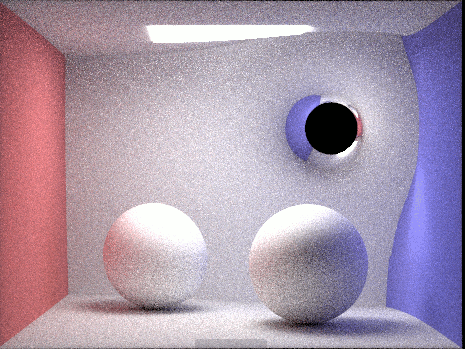
\includegraphics[width=\linewidth]{lense.png}
  \caption{Black hole in Cornell Box. Note the bright spot on the blue wall as a result of the gravitational lensing}
  \Description{Black hole in Cornell Box. Note the bright spot on the blue wall as a result of the gravitational lensing}
\end{figure}

\section{Gravitational Redshift}

The distortion of spacetime induces changes in the local speed of light. Due to the wave nature of light, light spectra undergo a wavelength shift in a phenomenon known as gravitational redshift. Emission near the black hole becomes longer in wavelength as it moves away from the black hole and is described by the equation\cite{wikipedia_2019}:

\begin{displaymath}
  \frac{\lambda_1}{\lambda_2} = [(1 - r_s / R_1)(1 - r_s/R_2)]^{1/2}
\end{displaymath}

where $R_1, R2$ are the distances of the emitter and observer respectively relative to the black hole and $\lambda_1, \lambda_2$ are the emitted and observed wavelength respectively. In order to implement redshift, we took spectral data for the Cornell box and used spectral intensity values ranging from 400nm to 700nm with 4nm resolution\cite{cornell}.

\begin{figure}[h]
  \centering
  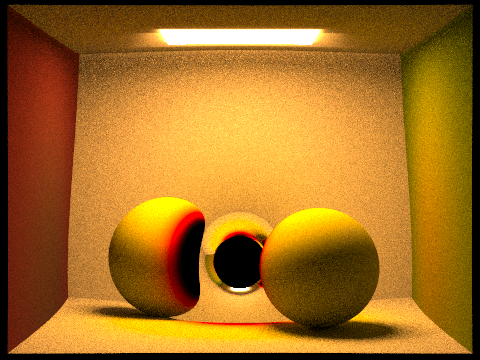
\includegraphics[width=\linewidth]{CBspheres_lambertian_screenshot_4-28_20-52-32.png}
  \caption{Black hole with redshift.  Note that the spheres appear black due to visible wavelengths being pushed out the visible range.  In addition, parts of the green wall appear more yellow-orange and the red wall more off red-grayish as a result of the redshift}
  \Description{}
\end{figure}

\section{Progress}

For our future goals, we would like to be able to implement a black hole with spin.  This would be very hard however as this requires solving 5 differential equations simultaneously numerically.  We can also see about optimizing our code to run on a GPU through CUDA or OpTix.

\section{Acknowledgments}

Special thanks to the Open Computing Facility (ocf.io) for letting us run our CPU intensive ray tracer. And Ren Ng for answering our questions regarding color spaces and where to find spectral data.

\bibliographystyle{ACM-Reference-Format}
\bibliography{paper}


\end{document}
